%%%%%%%%%%%%%%%%%%%%%%%%%%%%%%%%%%%%%%%%%%%%%%
%                insertmeeting
% 1) Title (something creative & funny?)
% 2) Date (MM/DD/YYYY)
% 3) Location (ex. Hagerty High School)
% 4) People/Committees Present 
% 5) Picture 
% 6) Start Time & Stop Time (ex. 12:30AM to 4:30PM)
%%%%%%%%%%%%%%%%%%%%%%%%%%%%%%%%%%%%%%%%%%%%%%
\insertmeeting 
  {Post Meet Cleanup} 
  {01/18/22} 
  {Hagerty High School}
  {Jensen}
  {Images/RobotPics/robot.jpg}
  {2:30 - 4:30}
  
\hhscommittee{General}
\noindent\hfil\rule{\textwidth}{.4pt}\hfil
\subsubsection*{Goals}
\begin{itemize}
    \item Reorganize all supplies from last meet and put tools back into the room

\end{itemize} 

\noindent\hfil\rule{\textwidth}{.4pt}\hfil

\subsubsection*{Accomplishments}
Our most recent Space Coast League Meet was Saturday 1/15/22. Because of this, a lot of our team's supplies were on the mentors' cars. Our first priority was moving everything back to the robotics room for use until the League Championships. Because our school is hosting the League championships, we also had to store fields for use on competition day. 



\hhscommittee{Multimedia}
\noindent\hfil\rule{\textwidth}{.4pt}\hfil
\subsubsection*{Goals}
\begin{itemize}
    \item Make progress on the backgrounds for the FLL and FTC themed scenes.

\end{itemize} 

\noindent\hfil\rule{\textwidth}{.4pt}\hfil

\subsubsection*{Accomplishments}
After debriefing about our progress over the past few days, we started drawing again. We have learned to split the work between two background artists, someone to draw characters, another to color them, and a video editor. This way none of the members working on the video will get burnt out or have to complete tasks that are overwhelming. Now while drawing the frames for FLL, we wanted to incorporate our own experience with FLL mentoring. We did this by drawing an environment that resembles our school's media center, where we host our meetings. We also included the circular table where we typically host our meetings for the Discover students. We chose green to represent how being a part of FLL was a fresh, new beginning for the students. Then, for the FTC scenes, we heavily incorporated our own robotics room, including defining aspects like the shelving on the back wall and the rolling carts that we use to hold our supplies. These additions add a personal touch to the scenes, making it unique to our team while still effectively depicting the theme of the Promote video.

\begin{figure}[ht]
\centering
\begin{minipage}[b]{.48\textwidth}
  \centering
  
\includegraphics[width=0.95\textwidth]{Meetings/January/01-18-22/1.18.22_ - Falon Jones.png}
  \caption{A Promote video background}
  \label{fig:010822_1}
\end{minipage}%
\hfill%
\begin{minipage}[b]{.48\textwidth}
  \centering
  
\includegraphics[width=0.95\textwidth]{Meetings/January/01-18-22/1.18.22 - Falon Jones.png}
  \caption{Another background}
  \label{fig:010822_2}
\end{minipage}
\end{figure}

\begin{figure}[htp]
\centering
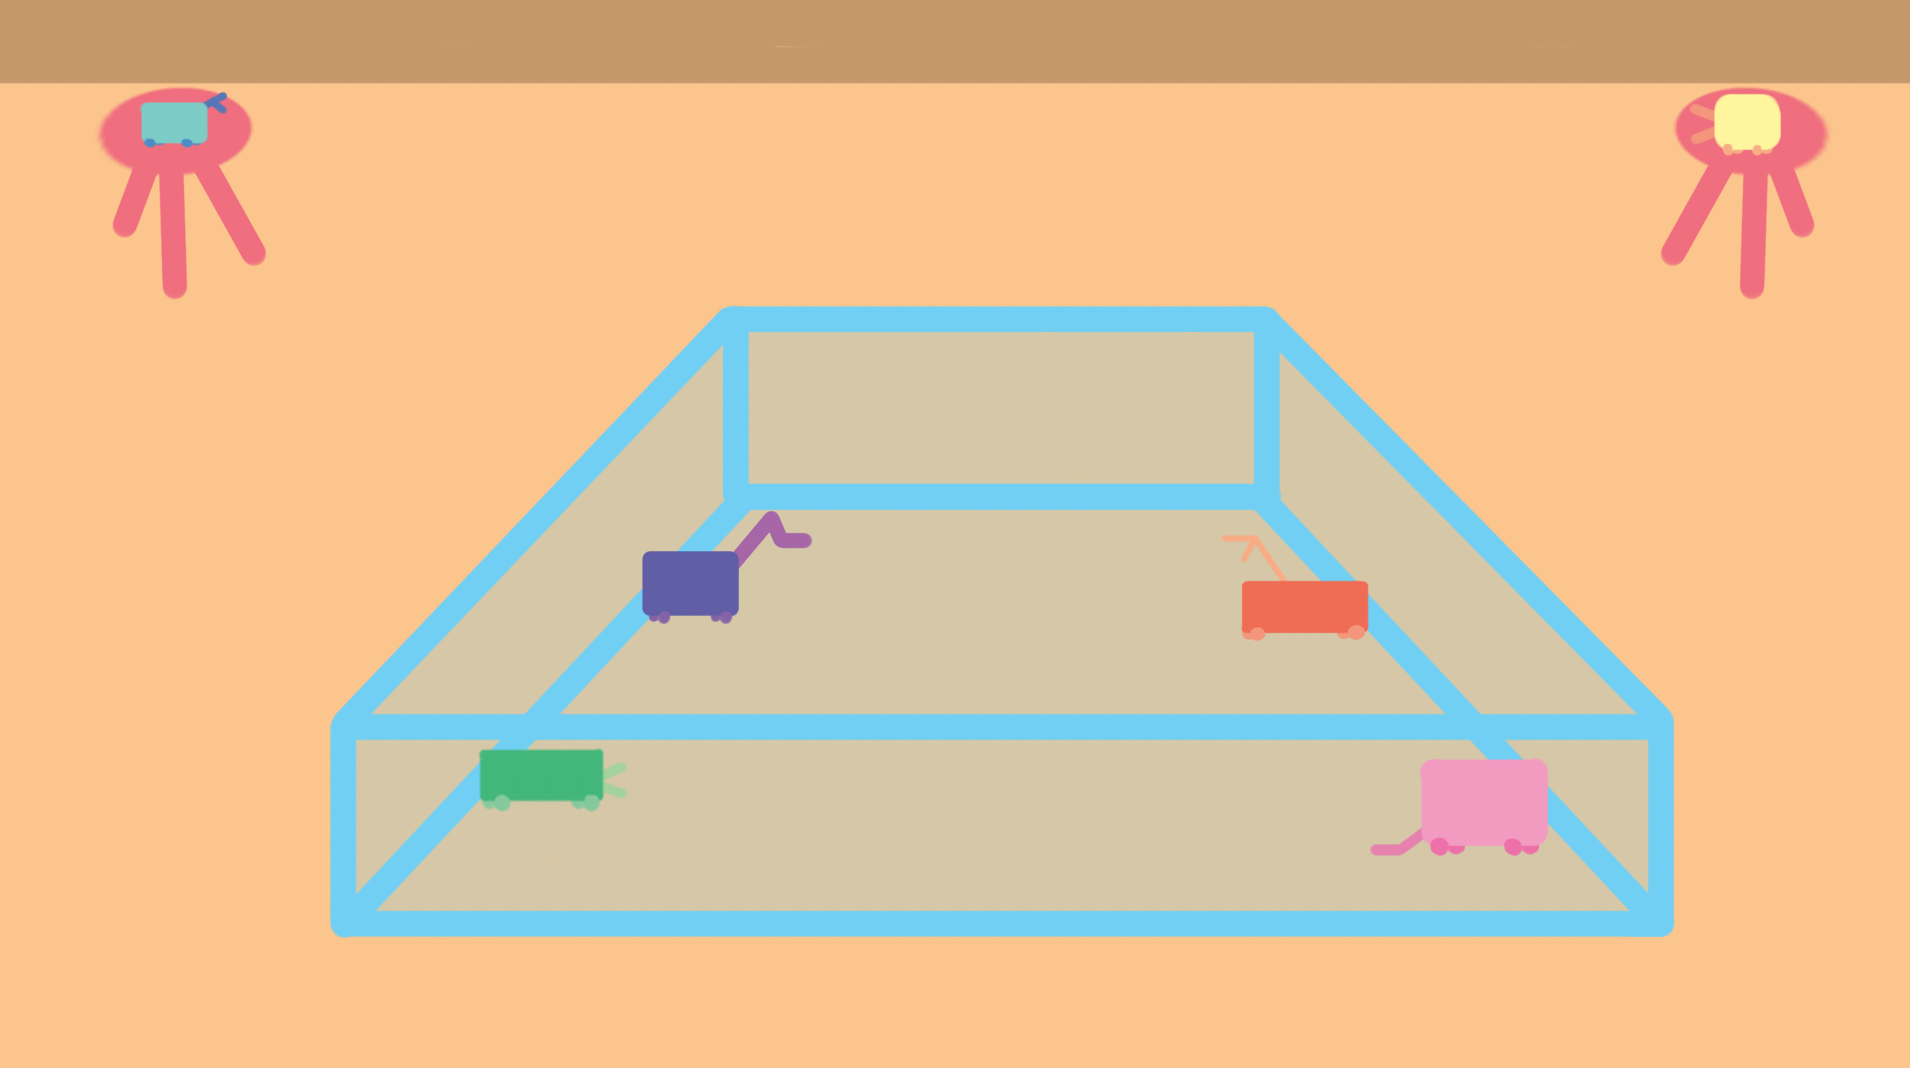
\includegraphics[width=0.95\textwidth, angle=0]{Meetings/January/01-18-22/1.18.22- - Falon Jones.png}
\caption{A third Promote video background}
\label{fig:010822_3}
\end{figure}


\whatsnext{
\begin{itemize}
    \item Complete all background frames and begin character drawing.
\end{itemize} 
}

